\documentclass[a4paper,11pt]{article}

\usepackage{amssymb}
\usepackage{amstext}
\usepackage{amsmath}
\usepackage{amsthm}
\usepackage{booktabs}
\usepackage{graphicx}
\usepackage{float}
\usepackage{url}

\usepackage{xcolor}
\newcommand{\bluenote}[1]{\color{blue}{ \em #1 }\color{black}}

\usepackage{geometry}
 \geometry{
 a4paper, %letterpaper,
 total={17cm,22.8cm},
 margin=24mm,
 top=22.4mm,
 bottom=25.4mm
 }
 
% Times new roman
\usepackage{mathptmx}

\usepackage[T1]{fontenc}

\thispagestyle{empty} 

\setlength{\parindent}{0pt}

% For comment boxes.
\usepackage[colorinlistoftodos,prependcaption,textsize=tiny]{todonotes}
\newcommand{\giselle}[1]{\todo[linecolor=red,backgroundcolor=red!25,bordercolor=red]{G: #1}}
\newcommand{\samar}[1]{\todo[linecolor=blue,backgroundcolor=blue!25,bordercolor=red]{S: #1}}

\author{%
%  \fontsize{10}{12}\selectfont
  \begin{minipage}[t]{0.47\textwidth}
    \centering
    Samar Rahmouni \\ srahmoun@andrew.cmu.edu
  \end{minipage}
  \and
  %
  \begin{minipage}[t]{0.45\textwidth}
    \centering
    Advisor: Prof. Giselle Reis \\ giselle@cmu.edu
  \end{minipage}%
  \vspace*{2ex}
}


\date{}

\title{{\Large\sc Senior Thesis 2021-22\\[2ex]}{\LARGE\bf Mid-Semester Report\vspace*{3ex}}}


\begin{document}

\maketitle 

\textcolor{red}{To redo, don't read.}
\begin{abstract} Reinforcement learning (RL), though a powerful and simple trial-and-error procedure that found a lot of success in games like Go, cannot be deployed in the real world 
because of the lack of security guarantees. For instance, though an autonomous car trained with reinforcement learning is bound to learn how to drive, the AI needs to crash 
to learn that crashing is not desirable. 

\medskip

In the context of the proposed thesis, we investigate both the security and the interpretability aspect of reinforcement learning in a cooperative adaptive cruise control inspired from \cite{vnc20},
in the aim of finding how formal security frameworks can guide the representation, robustness and extrapolation of knowledge in reinforcement
learning agents. We do so by experimenting and comparing both the optimization and security of three different RL implementations. 

\medskip

The first is a basic tabular Q-learning where we expect no security guarantees. The second is a hybrid architecture that incorporates the safe controller in \cite{vnc20} in a RL architecture. 
The safe controller (SC) computes a range of safe velocities given the current state of the environment in the car platooning scenario. Precisely, for multiple vehicles following each other, platooning aims to reduce the distance between them, hence taking less space on the road 
and allowing more vehicles to occupy highways, for instance. In the RL architecture, the SC then constricts the possible actions of the RL continuously at every given time step and the role of the RL is purely 
to find the optimal velocity in the safe range to minimize the distance between the cars. The third is what we will define as a logic-based inference RL. We investigate learning inferences rules in a deterministic environment 
where the result of an action given a state is not dependent on any probabilistic event. We approach the problem using inductive reasoning where the goal is to incorporate the learned rule knowledge into the decision making of a tabular Q-learning RL agent. 
In the given scenario, this will make use of the SC to develop a mapping from the state representation to a reward scheme, i.e. punish before a crash is bound to happen and adapt the Q-value and the epsilon-greedy approach. 
\end{abstract}


{\color{red}Writing rules (by Giselle Reis):
\begin{itemize}
  \item Each sentence must be a natural continuation of the next, reusing
  the same words and concepts. This ensures a natural reading flow.
  \item Crucial concepts are emphasized when they appear for the first
  time.
  \item Information is given in a \emph{by need} basis. Don't overload
  the reader with more information than necessary at any given point.
\end{itemize}
}

\newpage

\section{Introduction}
Implementing a robust adaptive controller that is effective in terms
of precision, time, and quality of decision
when facing dynamic and uncertain scenarios, has always been a central
challenge in AI and robotics. Precisely, as we want our autonomous agents to be deployed 
in the real world, we want to ensure that they are able to adapt to unforeseen scenarios, as well as 
keep their efficiency. This efficiency is measured in terms of their optimality and time taken to produce a decision. 
%
As autonomous cars are deployed, IoT is popularized, and human-robot interactions become more complex, we
are more and more confronted with the need for robotic agents that can effectively and continually adapt
to their surroundings, not only in simulation, but also in practice, when deployed as a cyber-physical system. 
Since we are unable to provide a repertoire of all possible scenarios and actions,
our agents need to be able to autonomously predict and adapt to new
changes. Reinforcement Learning (RL) is an approach that
supports dynamically adapting to new input. It is also the solution that AlphaGo, Deepmind AlphaStar, and OpenAI Five have
adopted \cite{li2019reinforcement}, respectively for Go, StarCraft II and Dota 2 and found success in. 

\medskip

Reinforcement Learning is a powerful tool as it does not require pre-gathered data as most Machine Learning (ML) 
techniques do. The general idea of RL is a trial-and-error process. In other words, a car trained using RL is bound to 
crash to learn not to crash again. This learning is based around a \textit{domain dependent} reward function. For example, say we want to teach an autonomous car to stop at a STOP sign. We will 
punish it via a negative reward when it does not, otherwise, we will reward it. Thus, through multiple iterations, 
and with the goal to maximize its rewards, a reinforcement learning trained agent will learn to stop at a STOP sign. 
%

\medskip

The task of choosing a reward function that ensures optimality is thus crucial. In the following work, we propose a Domain Informed Oracle (DIO) to
inform a reinforcement learning . Precisely, we propose a systematic way to encode domain specific rules into a reward function for RL. We argue that such a combination will ensure 
a faster and more efficient RL trained agent in terms of optimality. The proposed combination is then tested on a traffic simulation. The results are compared with 
a RL implementation that makes use of standard practices to design a reward function. 



\section{Reinforcement Learning} 
Reinforcement Learning is a method of learning that maps situations to
actions in order to maximize its rewards
\cite{sutton2018reinforcement}. Rewards are numerical values associated to a state and action. Precisely, one defines a reward function 
$R : (S * A) \rightarrow \mathbb{R}$ where $S$ defines the state space and $A$ the action space. Note that a state refers to the current configuration
of the environment and the action refers to the action chosen by the RL agent. By defining this reward function and the scenario of the problem the agent is trying to solve, 
reinforcement learning has the advantage of not requiring a prior dataset. Indeed, the agent is not told what to do, but rather 
learns from the effect of its actions on the environment. Consider figure \ref{fig:rl}. 
\begin{figure}[H]
  \centering
  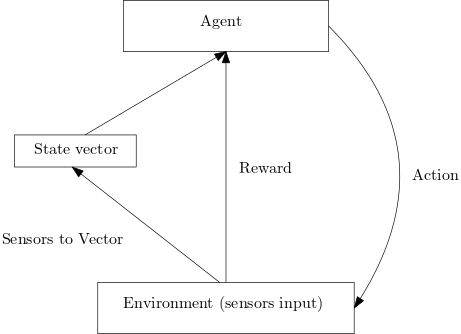
\includegraphics[scale=0.6]{rlroutine.png}
  \caption{Reinforcement Learning Routine}
  \label{fig:rl}
\end{figure}


The diagram in Figure~\ref{fig:rl} is a high-level description of how
an agent using reinforcement learning can be trained.  
%
The lower box represents the \emph{environment} as seen by the agent
according to its sensors.
%
The current state of the environment is represented as a \emph{state
vector}.
%
At each iteration, the agent will receive the state vector as input,
and needs to choose an \emph{action} to take.
%
Once the action is taken, the environment is updated to the next state
and the agent receives a \emph{reward} as feedback.
%
This reward is a domain dependent function that represents how
``good'' the state is.
%
The agent's goal is to increase its reward by taking actions that
reach better states each time.\giselle{This last sentence is like a
magic box to me. Maybe we need to make it less magic, maybe not.}\samar{I think it's fine to 
keep it as a black box. It will involve mentioning Bayesian and Markov decision process and 
I didn't need those in the latter half.} 
%

\medskip 

The reward function is a crucial aspect of the RL algorithm. For instance, consider a game of chess 
where the agent is punished when it loses and rewarded if it wins. The agent is bound to learn how to 
maximize its winnings but it will need to exhaust multiple possible combinations to learn. In this case, 
the training time is not optimal. A better approach would be to also reward it for making a good opening, for instance. 
Another example would be only considering negative rewards. Say we want our agent to escape a maze, and we punish it at every timestep for not escaping. 
If there is a 'fire'/fatality state, the agent will learn to move towards the fatality state as to cut its negative rewards as soon as possible. 
In conclusion, a good reward function is the first step of optimal learning. By choosing the right reward function, 
we can ensure a faster and more efficient training, possibly with fewer errors. 

\section{Challenges in Reinforcement Learning}

\subsection{Reward Shaping}
The task of choosing a reward function that ensures optimality is thus crucial. However, the generation of an appropriate 
reward function for a given problem is still an open challenge \cite{kober2013}. This problem is known as \textit{Reward Shaping} \cite{laud2011}.  
Ideally, rewards would be given by the real-world, i.e. \textit{native rewards}. For instance, recent work investigates dynamically generating a reward 
using a user verbal feedback to the autonomous agent \cite{gonzalez2010}. However, most RL agents 
can only stay in simulation due to the lack of safety guarantees. This is because of the trial-and-error nature of the RL training. 
Thus, there exists a need for \textit{shaping rewards} instead. There are reasonable criteria on how this should be done: \emph{standard practices}. \textcolor{red}{describe those practices}
However, there still exists a lack of a systematic method to design a reward function.

\subsection{Exploration vs. Exploitation}
A central issue in reinforcement learning is the dilemma of \emph{exploration} vs. \emph{exploitation}. Consider this problem. An agent is at an intersection. It has the choice of going either right or left. 
It does not yet know the outcome of either. It chooses right at a given point and receives a reward $r=1$. The question is "When faced with the same decision, should it keep going right?" There are two issues to consider. 
First, it does not know the outcome of going left. It could be that there is a better reward waiting for it on the left lane. Second, when dealing with a stochastic environment, it might be that $r$ was a one-time occurence. 
It would be equivalent to someone buying a lottery ticket, and winning \$1M on their first try, and thus, spending all that their won in trying to make it happen again. This problem showcases the importance of exploration; an agent 
needs to see where other paths might lead to, but also exploitation; if it keeps exploring forever it will never accumulate rewards. This is especially evident when the possible states cannot be exhausted. Several techniques have been proposed 
to balance between exploration and exploitation \cite{Kaelbling1996ReinforcementLA}. A notable one is the \emph{epsilon-greedy} technique. The idea is to set some probability $\epsilon$ by which the agent decides to explore. This probability can be adapted 
to decrease as more \emph{episodes} are completed. 

\subsection{Meta-Learning}
The result of training is a policy $\pi$, a function to map states to action $\pi : S \rightarrow A$. The learned policy is the one that maximizes the cumulative rewards.
This training is most often done in simulation, given the lack of safety guarantees of RL. 
However, several problems come into place when considering the deployment of the trained agent. Considering that an agent has done well in 
a designed simulation does not imply that it will do as well in the real-world. Overall, it must be that certain uncertainties will not be expected, thus there can be no expectation on how the agent will behave 
when out of simulation. This problem of adaptation is known as \emph{Meta-learning}. Meta-learning in reinforcement learning is the problem of learning-to-learn, which is about efficiently
adapting a learned policy to conditions and tasks that were not encountered in the past. In RL, meta-learning
involves adapting the learning parameters, balancing exploration and exploitation to direct the
agent interaction \cite{gupta_meta-reinforcement_2018,schweighofer_meta-learning_2003}. Meta-learning is a central problem in AI, since an agent that can solve more
and more problems it has not seen before, approaches the ideal of a general-purpose AI. 


\section{Symbolic Reasoning for Reinforcement Learning}
As to tackle the challenges from section 3, we are inspired from current Neurosymbolic AI trends. Precisely, neurosymbolic integration has been an ongoing work in the last years towards a combination of deep learning (DL) and symbolic reasoning.
The work has been a response to criticism of DL on its lack of formal semantics and intuitive explanation and the lack of expert knowledge towards guiding machine learning models. 
Key questions the field targets are identifying the necessary and sufficient building blocks of AI \cite{garcez2020neurosymbolic}, namely, how can we provide the semantics of knowledge, 
and work towards meta-learning? 

Current Neurosymbolic AI trends are concerned with knowledge representation and reasoning, namely, they investigate computational-logic systems 
and representation to precede learning in order to provide some form of incremental update, e.g. a meta-network to group two sub-neural networks. \cite{Besold2017NeuralSymbolicLA}
This leads to neurosymbolic AI finding various applications including vision-based tasks such as semantic labeling \cite{vinyals2015, karpathy2015}, 
vision analogy-making \cite{Reed2015DeepVA}, or learning communication protocols \cite{Foerster2016LearningTC}. Those results inspire us to use those techniques for reinforcement learning, as to tackle its challenges.

\medskip
Rewards are domain dependent and thus, given domain specific rules, a \emph{domain informed} module can guide a RL agent towards better decisions. This can be done by 
adapting the reward function by defining which states are desirable, which are to be avoided and which are fatal. Given rules and judgments, a logic programming module 
is able to search the space and send feedback to the reinforcement learning agent. The goal is a systematic method to design a reward function which can ensure faster and more efficient 
training. This knowledge can furthermore be incorporated into resolving the exploration vs. exploitation dilemma, \textcolor{red}{how tho}
We will call the propose module a \emph{Domain Informed Oracle (DIO)}. 

\begin{figure}[H]
  \centering
  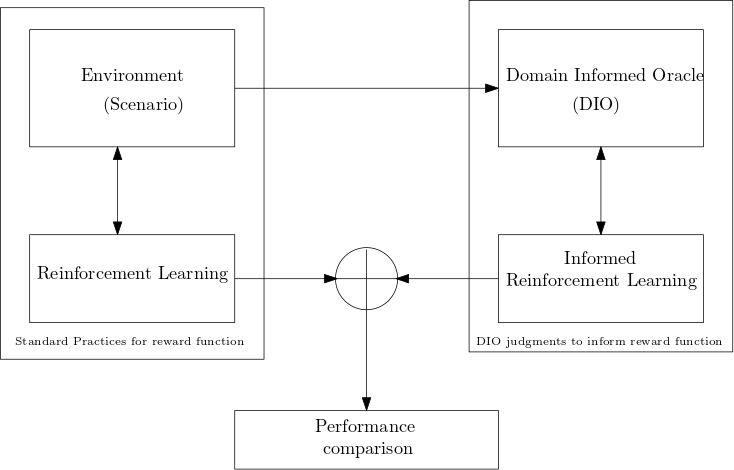
\includegraphics[scale=0.6]{overview.png}
  \caption{Overview of the proposed solution}
  \label{fig:overview}
\end{figure}

The diagram in Figure~\ref{fig:overview} is a high-level description of our proposed solution. 
%
The box on the left represents a basic reinforcement learning algorithm that depends on the scenario of the given problem and 
the common standard practices discussed previously to design a reward function. 
%
The box on the right represents our proposed domain knowledge to inform the reinforcement learning algorithm. 
Precisely, the domain informed oracle is given the scenario and can thus start a feedback loop between itself and 
the informed RL module to update the rewards. 
%
Finally, those two implementations will be compared based on their performance. In the following, we define performance 
given three metrics: (1) time to train (2) optimality of the learned policy and (3) number of errors through training. 
Consider 'errors' as suboptimal decisions that were made by the agent while in the process of training. For example, exploring a (state, action) pair 
that has previously given a negative reward is suboptimal. 

\section{Domain Informed Oracle} 
\subsection{Architecture}
In this section, we lay the foundations of the architecture that combines the Domain Informed Oracle with 
reinforcement learning. Note that in our proposed architecture, we suppose Q-learning, a specific method to compute the policy in RL. 

\medskip 

\begin{figure}[H]
  \centering
  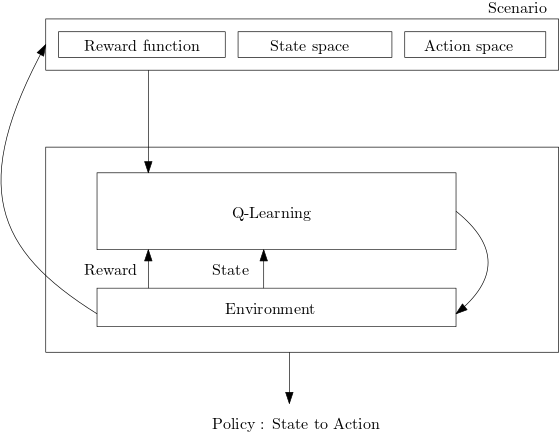
\includegraphics[scale=0.55]{basicrl.png}
  \caption{Reinforcement learning architecture}
  \label{fig:basicrl}
\end{figure}


\begin{figure}[H]
  \centering
  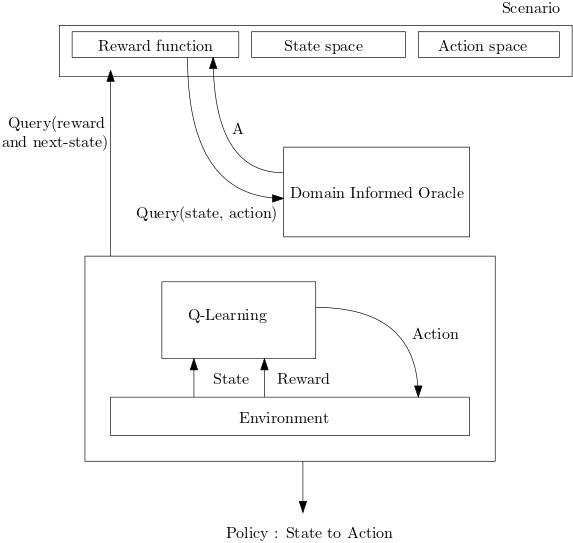
\includegraphics[scale=0.55]{dio.png}
  \caption{Dio+RL architecture}
  \label{fig:diorl}
\end{figure}

The diagram in Figure \ref{fig:basicrl} describes the basic routine of RL in more details. The environment, which as we follow a simulation is formalized in the scenario, sends the current state 
to the Q-Learning algorithm. The agent chooses an action from the action space and sends it to the environment. This action affects the environment that is then 
updated and the resulting state along its associated reward is computed from the reward function and step function formalized in the scenario. Thus, in the next iteration, the 
agent receives the reward from its previous action which it uses to improve its policy and continues with its training starting from the next state.  

\medskip 

The architecture in Figure \ref{fig:diorl} introduces DIO in the feedback loop. It is kept independent of the RL module. Precisely, when the scenario is query-ed for the reward and 
the resulting next state of a (state, action) pair, rather than computing the reward using the reward function, the latter is able to query DIO. The result of this query is $A$ which we keep 
obscure. The fundamental idea is that $A$ is used to inform the reward function when it is tasked with computing the reward. 

\subsection{Specifications} \label{scspecs}
DIO is a logic programming based module that takes the query from the reward function and returns $A$, a judgment that the scenario awaits to update its reward function. The judgment is obscured as it is a choice of the scenario, 
independent of the DIO implementation. In the following, we will define $A$ by its behavior, rather than its type. To do so, we will walk through the routine in the diagram of Figure \ref{fig:diospecs}.


\begin{figure}[H]
  \centering
  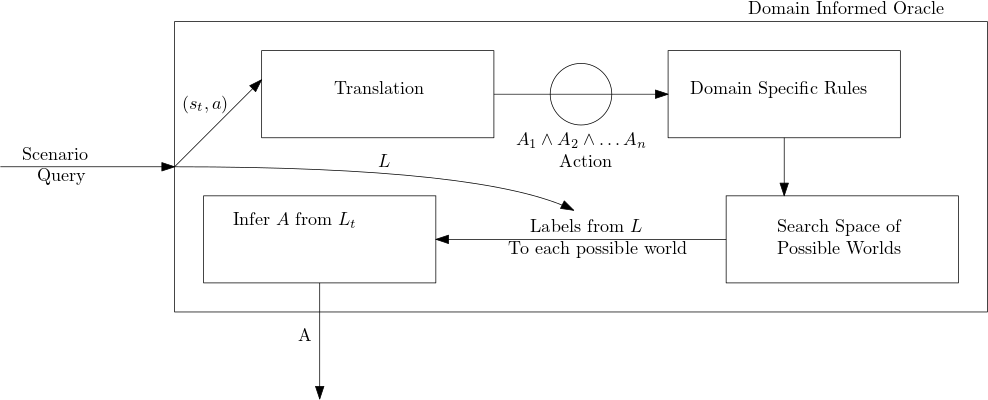
\includegraphics[scale=0.46]{diospecs.png}
  \caption{Domain Informed Oracle routine}
  \label{fig:diospecs}
\end{figure}

\begin{enumerate}
  \item The scenario queries DIO. It sends $(s_t, a)$, the state at time $t$ and the action. It also sends $L : s \rightarrow t$ where $t$ is a sum of types: 
        $t \equiv t_1 + t_2 .. + t_n$. For instance, consider our previous example of the chess game and let the scenario define good openings as "desirable" and random openings as 
        "undesirable". Thus $t \equiv d + ud$ where $d$ is equivalent to desirable and $ud$ to undesirable. 
  \item The first step of DIO is translation $T : \mathbb{R}^n \rightarrow t_1 \times t_2 \times ... t_n$ that takes in the state vector $s_t$ and returns a conjunction of propositions, let it be $P$. 
  \item P is passed alongside the action to the domain specific rules defined in DIO. 
  \item Using step semantics, DIO generates possible worlds up to a given time $t'$. Note that given the stochasticity of the environment, there is not certainty on
        whether the worlds expected by DIO will necessarily happen. 
  \item Those possible worlds, equivalent to states, can be transformed using $L$ to $t$. 
  \item At the last step, DIO ends up with a set $S$ of $t$ that defines the labels of all the possible worlds.
  \item The last step is left as an inference depending on how the the judgment for deciding a final $A$ from $S$ 
        is formulated. For instance, we can consider a rule where if most of the possible worlds are undesirable, then let $A$ be undesirable.
  \item Finally, $A$ is passed to the scenario. Note then that $A : t$. 
\end{enumerate}

Note how this does not guarantee that the reward function will be informed in a meaningful way.
To that end, we need to consider (1) what are the specifications of a 'good' reward function, (2) what conditions should be set 
on the domain specific rules and $L$ provided by the scenario, (3) how to define a systematic way for the scenario to use 
this information. Those considerations are left for future investigations. 

 

\section{Traffic Simulation} \label{traffic}


\section{Related Work}

take related work from prof. giselle notes

\section{Conclusions}
\textcolor{red}{todo.}

\newpage

\bibliographystyle{unsrt}
\bibliography{biblio.bib}

\newpage

\section{Appendix}



\end{document}
